\section{Diagrams}
\label{app:diagrams}
\begin{figure}[ht]
    
\usetikzlibrary{bayesnet, positioning}

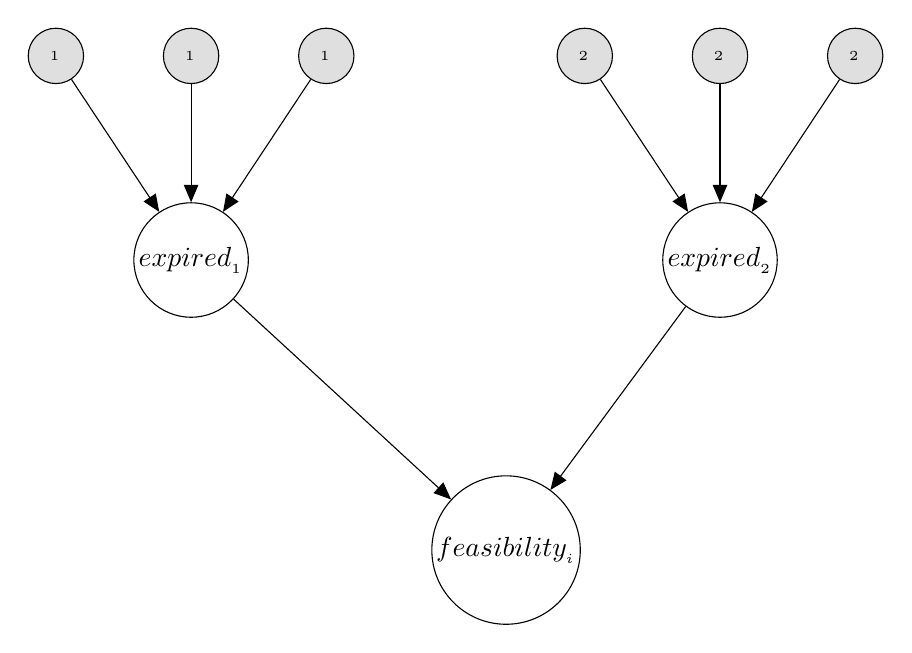
\begin{tikzpicture}
% --- Food 1 --- 
\node[obs] (ft1) {$\fty_{\food_1}$};
\node[obs, right=of ft1] (st1) {$\sty_{\food_1}$};
\node[obs, right=of st1] (d1) {$\days_{\food_1}$};
\node[latent, below=1.5cm of st1] (exp1) {$expired_{\food_1}$};

\edge {ft1, st1, d1} {exp1}

%--- Food 2 ---
\node[obs, right=6cm of ft1] (ft2) {$\fty_{\food_2}$};
\node[obs, right=of ft2] (st2) {$\sty_{\food_2}$};
\node[obs, right=of st2] (d2) {$\days_{\food_2}$};
\node[latent, below=1.5cm of st2] (exp2) {$expired_{\food_2}$};

\edge {ft2, st2, d2} {exp2}

%--- Feasibility node ---
\node[latent, below=2cm of exp1, xshift=4cm] (feas) {$feasibility_{\recipe_i}$};

\edge {exp1, exp2} {feas}

\end{tikzpicture}


    \caption{Bayesian Network Structure}
    \label{fig:BN}
\end{figure}

\begin{figure}[ht]
    \centering
    \includegraphics[width=1.0\textwidth]{appendix/Image/Decision-Network.png}
    \caption{Decision Network Structure}
    \label{fig:DN}
\end{figure}

\newpage

\section{Data}
\label{app:data}
\begin{itemize}
    \item attributes of recipe vector:
    'preparation', 'time-to-make', 'course', 'main-ingredient', 'dietary', 'easy', 'occasion', 'cuisine', 'low-in-something', '60-minutes-or-less', 'main-dish', 'equipment', '30-minutes-or-less', 'number-of-servings', 'meat', '4-hours-or-less', 'desserts', 'vegetables', '3-steps-or-less', 'taste-mood', 'north-american', 'low-sodium', 'low-carb', 'healthy', '15-minutes-or-less', 'step\_cnt', 'ingredient\_cnt'

    \item Training data for Utility function: \href{https://www.kaggle.com/datasets/realalexanderwei/food-com-recipes-with-ingredients-and-tags}{Kaggle — Food.com Recipes with Ingredients and Tags}
    \item Training data for Bayesian Network: \href{https://github.com/CS3263-Group66/Group66-Project/blob/main/Code/Data/food_condition.csv}{GitHub — food\_condition.csv}
\end{itemize}

\newpage

\section{Algorithm}
\label{app:algorithm}
\subsection{Algorithms for inference machine}
\input{appendix/algorithms/algo1}

\newpage

\section{Contribution}
Lei Jianwen: 
\begin{itemize}
    \item Agent Structure design.
    \item Sub-Bayesian Network for food expiration model.
    \item Integration between front end and backend.
\end{itemize}

San Muyun:
\begin{itemize}
    \item Building of SmartFridge CLI app.
    \item Integration between various models and utility.
    \item Integrate the models and functions into the CLI app.
    \item Analyze the section on responsible AI.
\end{itemize}

Chen Yixun: 
\begin{itemize}
    \item Training the model for Utility function.
    \item Data collection and analysis.
    \item Implementing the Bayesian Network and mechanism of inference.
    \item System and architecture design.
\end{itemize}

\section{Acknowledgment of the use of Generative AI}
We utilized Generative AI tools primarily to understand APIs of libraries used such as \textbf{pgmpy} and \textbf{scikit-learn}, and learn Latex syntax and packages to format and generate the report. The main design and implementation of different components of the application were done independently. AI tools were only used as reference and learning aids to become familiar with tools and syntax 